% This file was created by matlab2tikz.
%
%The latest updates can be retrieved from
%  http://www.mathworks.com/matlabcentral/fileexchange/22022-matlab2tikz-matlab2tikz
%where you can also make suggestions and rate matlab2tikz.
%
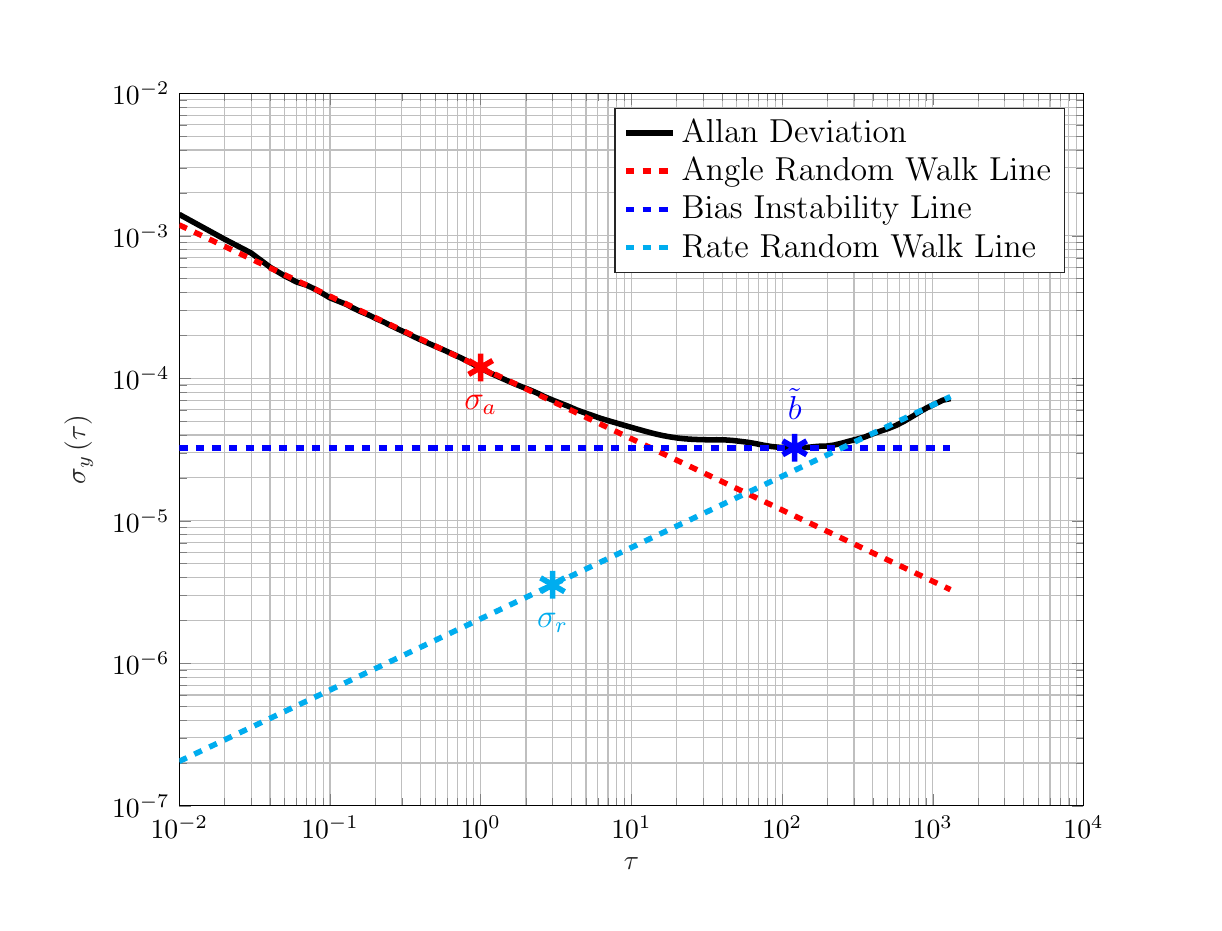
\begin{tikzpicture}

\begin{axis}[%
width=4.521in,
height=3.563in,
at={(0.758in,0.484in)},
scale only axis,
xmode=log,
xmin=0.01,
xmax=10000,
xminorticks=true,
xlabel style={font=\color{white!15!black}},
xlabel={$\tau$},
ymode=log,
ymin=1e-07,
ymax=0.01,
yminorticks=true,
ylabel style={font=\color{white!15!black}},
ylabel={$\sigma_y\left(\tau\right)$},
axis background/.style={fill=white},
xmajorgrids,
xminorgrids,
ymajorgrids,
yminorgrids,
legend style={legend cell align=left, align=left, draw=white!15!black}
]
\addplot [color=black, line width=2.0pt]
  table[row sep=crcr]{%
0.01	0.00141284849914709\\
0.02	0.000946173025243918\\
0.03	0.000757071812060535\\
0.04	0.00060278142970404\\
0.05	0.00052350772762438\\
0.06	0.000474252115240417\\
0.07	0.000450382779750475\\
0.08	0.000421041567730099\\
0.09	0.000392076706028194\\
0.1	0.000366942086447977\\
0.11	0.000352506262463209\\
0.13	0.00032841350662045\\
0.14	0.000314108985701804\\
0.16	0.000293641373932674\\
0.18	0.000278713939983907\\
0.2	0.000263659663850093\\
0.23	0.000246968855165468\\
0.25	0.000235959914132601\\
0.29	0.000218875735183774\\
0.32	0.000208688893932888\\
0.36	0.000196079274116195\\
0.41	0.00018400863139319\\
0.46	0.000174232859102089\\
0.51	0.000166022632656421\\
0.58	0.000156618684503399\\
0.65	0.00014818443593899\\
0.73	0.000140075832803897\\
0.82	0.000131654666795674\\
0.93	0.000122716593172211\\
1.04	0.000115352961088433\\
1.17	0.000108392911144895\\
1.32	0.000102227741418525\\
1.49	9.65784535600634e-05\\
1.68	9.14462228936811e-05\\
1.89	8.6882519325959e-05\\
2.12	8.29748582463672e-05\\
2.39	7.84854249205103e-05\\
2.69	7.39073284008203e-05\\
3.03	7.00875303510261e-05\\
3.42	6.66266583875158e-05\\
3.85	6.34282403109679e-05\\
4.33	6.00596582028683e-05\\
4.88	5.73749596002113e-05\\
5.5	5.49291194162197e-05\\
6.19	5.25486396786345e-05\\
6.97	5.05830826556052e-05\\
7.85	4.87747361232601e-05\\
8.84	4.69898369308114e-05\\
9.96	4.53353046173432e-05\\
11.22	4.37487798674715e-05\\
12.64	4.22366375171173e-05\\
14.24	4.08668597821236e-05\\
16.03	3.9725958063853e-05\\
18.06	3.88167009343418e-05\\
20.34	3.80941714790052e-05\\
22.91	3.76005290552967e-05\\
25.81	3.73001853757038e-05\\
29.07	3.71215416665767e-05\\
32.74	3.70284209901191e-05\\
36.88	3.70631342754961e-05\\
41.54	3.69922326489072e-05\\
46.79	3.6663532195709e-05\\
52.71	3.61462578921871e-05\\
59.37	3.55784612366481e-05\\
66.87	3.48148151226476e-05\\
75.32	3.39359768494114e-05\\
84.84	3.32364425113324e-05\\
95.57	3.2823962521296e-05\\
107.65	3.26633725111685e-05\\
121.25	3.25433514505585e-05\\
136.58	3.25509851440239e-05\\
153.84	3.29382327306858e-05\\
173.28	3.33532061651855e-05\\
195.19	3.34372488367563e-05\\
219.86	3.39821975898702e-05\\
247.65	3.49995726524067e-05\\
278.95	3.62493790336099e-05\\
314.2	3.74435302804389e-05\\
353.92	3.87671546993383e-05\\
398.65	4.07362535999729e-05\\
449.04	4.25592484483615e-05\\
505.8	4.43810149818136e-05\\
569.73	4.66826103434735e-05\\
641.74	4.98001850295669e-05\\
722.86	5.35777660778605e-05\\
814.23	5.79056522743863e-05\\
917.14	6.22350656429574e-05\\
1033.07	6.60000445441277e-05\\
1163.64	7.01919867938027e-05\\
1310.73	7.20880028887797e-05\\
};
\addlegendentry{\large Allan Deviation}

\addplot [color=red, dashed, line width=2.0pt]
  table[row sep=crcr]{%
0.01	0.00119160083000573\\
0.02	0.000842589027364573\\
0.03	0.000687971059970392\\
0.04	0.000595800415002867\\
0.05	0.000532900091587598\\
0.06	0.000486469001765161\\
0.07	0.000450382779750475\\
0.08	0.000421294513682286\\
0.09	0.000397200276668578\\
0.1	0.000376817268456523\\
0.11	0.000359281168455008\\
0.13	0.000330490607113163\\
0.14	0.000318468717691208\\
0.16	0.000297900207501433\\
0.18	0.000280863009121524\\
0.2	0.000266450045793799\\
0.23	0.000248465948858569\\
0.25	0.000238320166001147\\
0.29	0.00022127471909997\\
0.32	0.000210647256841143\\
0.36	0.000198600138334289\\
0.41	0.000186096784291581\\
0.46	0.000175691957331844\\
0.51	0.000166857491036828\\
0.58	0.000156464854380738\\
0.65	0.000147799892686042\\
0.73	0.000139466328143732\\
0.82	0.000131590298129587\\
0.93	0.000123563250011663\\
1.04	0.000116846074704088\\
1.17	0.000110163535704388\\
1.32	0.000103715539661131\\
1.49	9.7619743645768e-05\\
1.68	9.1933999943747e-05\\
1.89	8.66762063757695e-05\\
2.12	8.18394810056567e-05\\
2.39	7.70782501400092e-05\\
2.69	7.26531848691921e-05\\
3.03	6.84556790458727e-05\\
3.42	6.44343933547088e-05\\
3.85	6.07296016327166e-05\\
4.33	5.72646814090765e-05\\
4.88	5.39412350647267e-05\\
5.5	5.08100301134325e-05\\
6.19	4.78944811183911e-05\\
6.97	4.51350998954102e-05\\
7.85	4.25300573827657e-05\\
8.84	4.00778729824141e-05\\
9.96	3.77573171459865e-05\\
11.22	3.55741366183515e-05\\
12.64	3.35163919143215e-05\\
14.24	3.15773588404974e-05\\
16.03	2.97621318183782e-05\\
18.06	2.80396071127583e-05\\
20.34	2.64213693837631e-05\\
22.91	2.48953509240181e-05\\
25.81	2.34550733144971e-05\\
29.07	2.21008145896969e-05\\
32.74	2.0825309261204e-05\\
36.88	1.96216416919479e-05\\
41.54	1.84883243229653e-05\\
46.79	1.74202456329416e-05\\
52.71	1.64128609038408e-05\\
59.37	1.5464905572758e-05\\
66.87	1.45718648775722e-05\\
75.32	1.37301613657631e-05\\
84.84	1.2936907327531e-05\\
95.57	1.21890540836804e-05\\
107.65	1.14848090789192e-05\\
121.25	1.08215612878564e-05\\
136.58	1.01961741095222e-05\\
153.84	9.60718517021759e-06\\
173.28	9.0522507890841e-06\\
195.19	8.52907660335181e-06\\
219.86	8.03632857757494e-06\\
247.65	7.57201788151048e-06\\
278.95	7.13456689237144e-06\\
314.2	6.72245194989609e-06\\
353.92	6.33400270353362e-06\\
398.65	5.96808380334227e-06\\
449.04	5.62326153049085e-06\\
505.8	5.29835903868121e-06\\
569.73	4.9922491625682e-06\\
641.74	4.70382593253243e-06\\
722.86	4.43204029616365e-06\\
814.23	4.17596881844575e-06\\
917.14	3.9347122689307e-06\\
1033.07	3.70736992113307e-06\\
1163.64	3.49318411220257e-06\\
1310.73	3.29135083265979e-06\\
};
\addlegendentry{\large Angle Random Walk Line}

\addplot [color=blue, dashed, line width=2.0pt]
  table[row sep=crcr]{%
0.01	3.25433514505585e-05\\
0.02	3.25433514505585e-05\\
0.03	3.25433514505585e-05\\
0.04	3.25433514505585e-05\\
0.05	3.25433514505585e-05\\
0.06	3.25433514505585e-05\\
0.07	3.25433514505585e-05\\
0.08	3.25433514505585e-05\\
0.09	3.25433514505585e-05\\
0.1	3.25433514505585e-05\\
0.11	3.25433514505585e-05\\
0.13	3.25433514505585e-05\\
0.14	3.25433514505585e-05\\
0.16	3.25433514505585e-05\\
0.18	3.25433514505585e-05\\
0.2	3.25433514505585e-05\\
0.23	3.25433514505585e-05\\
0.25	3.25433514505585e-05\\
0.29	3.25433514505585e-05\\
0.32	3.25433514505585e-05\\
0.36	3.25433514505585e-05\\
0.41	3.25433514505585e-05\\
0.46	3.25433514505585e-05\\
0.51	3.25433514505585e-05\\
0.58	3.25433514505585e-05\\
0.65	3.25433514505585e-05\\
0.73	3.25433514505585e-05\\
0.82	3.25433514505585e-05\\
0.93	3.25433514505585e-05\\
1.04	3.25433514505585e-05\\
1.17	3.25433514505585e-05\\
1.32	3.25433514505585e-05\\
1.49	3.25433514505585e-05\\
1.68	3.25433514505585e-05\\
1.89	3.25433514505585e-05\\
2.12	3.25433514505585e-05\\
2.39	3.25433514505585e-05\\
2.69	3.25433514505585e-05\\
3.03	3.25433514505585e-05\\
3.42	3.25433514505585e-05\\
3.85	3.25433514505585e-05\\
4.33	3.25433514505585e-05\\
4.88	3.25433514505585e-05\\
5.5	3.25433514505585e-05\\
6.19	3.25433514505585e-05\\
6.97	3.25433514505585e-05\\
7.85	3.25433514505585e-05\\
8.84	3.25433514505585e-05\\
9.96	3.25433514505585e-05\\
11.22	3.25433514505585e-05\\
12.64	3.25433514505585e-05\\
14.24	3.25433514505585e-05\\
16.03	3.25433514505585e-05\\
18.06	3.25433514505585e-05\\
20.34	3.25433514505585e-05\\
22.91	3.25433514505585e-05\\
25.81	3.25433514505585e-05\\
29.07	3.25433514505585e-05\\
32.74	3.25433514505585e-05\\
36.88	3.25433514505585e-05\\
41.54	3.25433514505585e-05\\
46.79	3.25433514505585e-05\\
52.71	3.25433514505585e-05\\
59.37	3.25433514505585e-05\\
66.87	3.25433514505585e-05\\
75.32	3.25433514505585e-05\\
84.84	3.25433514505585e-05\\
95.57	3.25433514505585e-05\\
107.65	3.25433514505585e-05\\
121.25	3.25433514505585e-05\\
136.58	3.25433514505585e-05\\
153.84	3.25433514505585e-05\\
173.28	3.25433514505585e-05\\
195.19	3.25433514505585e-05\\
219.86	3.25433514505585e-05\\
247.65	3.25433514505585e-05\\
278.95	3.25433514505585e-05\\
314.2	3.25433514505585e-05\\
353.92	3.25433514505585e-05\\
398.65	3.25433514505585e-05\\
449.04	3.25433514505585e-05\\
505.8	3.25433514505585e-05\\
569.73	3.25433514505585e-05\\
641.74	3.25433514505585e-05\\
722.86	3.25433514505585e-05\\
814.23	3.25433514505585e-05\\
917.14	3.25433514505585e-05\\
1033.07	3.25433514505585e-05\\
1163.64	3.25433514505585e-05\\
1310.73	3.25433514505585e-05\\
};
\addlegendentry{\large Bias Instability Line}

\addplot [color=cyan, dashed, line width=2.0pt]
  table[row sep=crcr]{%
0.01	2.05502606390325e-07\\
0.02	2.90624573060217e-07\\
0.03	3.55940955355871e-07\\
0.04	4.11005212780649e-07\\
0.05	4.59517797442148e-07\\
0.06	5.03376526468309e-07\\
0.07	5.43708790284392e-07\\
0.08	5.81249146120434e-07\\
0.09	6.16507819170974e-07\\
0.1	6.49856301294499e-07\\
0.11	6.81575038836799e-07\\
0.13	7.40950184581809e-07\\
0.14	7.68920345201656e-07\\
0.16	8.22010425561298e-07\\
0.18	8.71873719180651e-07\\
0.2	9.19035594884297e-07\\
0.23	9.85555877849645e-07\\
0.25	1.02751303195162e-06\\
0.29	1.10666540370759e-06\\
0.32	1.16249829224087e-06\\
0.36	1.23301563834195e-06\\
0.41	1.31585871983351e-06\\
0.46	1.39378648893149e-06\\
0.51	1.46758215541552e-06\\
0.58	1.56506122293237e-06\\
0.65	1.65681498066594e-06\\
0.73	1.75581503867145e-06\\
0.82	1.86090524775545e-06\\
0.93	1.98179536650209e-06\\
1.04	2.09572360015689e-06\\
1.17	2.22285055374543e-06\\
1.32	2.36104519287213e-06\\
1.49	2.50847899408173e-06\\
1.68	2.66361820972534e-06\\
1.89	2.82519374788313e-06\\
2.12	2.99216311411025e-06\\
2.39	3.17699319715022e-06\\
2.69	3.37049334841879e-06\\
3.03	3.57716232978945e-06\\
3.42	3.80040943343742e-06\\
3.85	4.03225230792772e-06\\
4.33	4.27623223106309e-06\\
4.88	4.53970095510814e-06\\
5.5	4.81946331848985e-06\\
6.19	5.11284537643777e-06\\
6.97	5.4254244902636e-06\\
7.85	5.75774149889304e-06\\
8.84	6.1100317487034e-06\\
9.96	6.48555286373366e-06\\
11.22	6.88357047059657e-06\\
12.64	7.30618847544914e-06\\
14.24	7.75483084509911e-06\\
16.03	8.22780699438473e-06\\
18.06	8.73325633124262e-06\\
20.34	9.26814476518158e-06\\
22.91	9.83625726307011e-06\\
25.81	1.04402605380772e-05\\
29.07	1.10800022935449e-05\\
32.74	1.17586285644862e-05\\
36.88	1.24799484256988e-05\\
41.54	1.32449578482826e-05\\
46.79	1.40570392348539e-05\\
52.71	1.49198288938005e-05\\
59.37	1.58343725534549e-05\\
66.87	1.68047863743197e-05\\
75.32	1.7834974391027e-05\\
84.84	1.89285638478626e-05\\
95.57	2.00899163021117e-05\\
107.65	2.13218238684119e-05\\
121.25	2.26286272220113e-05\\
136.58	2.40165648127136e-05\\
153.84	2.54889514466917e-05\\
173.28	2.70515126070462e-05\\
195.19	2.87108543786345e-05\\
219.86	3.04712623406629e-05\\
247.65	3.23397382540523e-05\\
278.95	3.43226267322386e-05\\
314.2	3.64267499668536e-05\\
353.92	3.86607154756092e-05\\
398.65	4.10311055293686e-05\\
449.04	4.35471612008907e-05\\
505.8	4.62175316084286e-05\\
569.73	4.90514532365765e-05\\
641.74	5.20591280067237e-05\\
722.86	5.52515455590547e-05\\
814.23	5.86395844866947e-05\\
917.14	6.22350656429575e-05\\
1033.07	6.60514277108369e-05\\
1163.64	7.01013941657513e-05\\
1310.73	7.44001745159338e-05\\
};
\addlegendentry{\large Rate Random Walk Line}

\addplot [color=red, line width=2.0pt, only marks, mark size=5.0pt, mark=asterisk, mark options={solid, red}, forget plot]
  table[row sep=crcr]{%
1	0.000119160083000573\\
};
\addplot [color=blue, line width=2.0pt, only marks, mark size=5.0pt, mark=asterisk, mark options={solid, blue}, forget plot]
  table[row sep=crcr]{%
121.25	3.25433514505585e-05\\
};
\addplot [color=green, line width=2.0pt, only marks, mark size=5.0pt, mark=asterisk, mark options={solid, cyan}, forget plot]
  table[row sep=crcr]{%
3	3.55940955355871e-06\\
};

%% DATA LABELS
\coordinate (N) at (axis cs: 1,0.000119160083000573);
\node[below, inner sep=0,yshift=-10,color=red]
at (N) {\large $\sigma_a$};
\coordinate (B) at (axis cs: 121.25,3.25433514505585e-05);
\node[above, inner sep=0,yshift=10,color=blue]
at (B) {\large $\tilde{b}$};
\coordinate (K) at (axis cs: 3,3.55940955355871e-06);
\node[below, inner sep=0,yshift=-10,color=cyan]
at (K) {\large $\sigma_r$};

\end{axis}

\begin{axis}[%
width=5.833in,
height=4.375in,
at={(0in,0in)},
scale only axis,
xmin=0,
xmax=1,
ymin=0,
ymax=1,
axis line style={draw=none},
ticks=none,
axis x line*=bottom,
axis y line*=left
]
\end{axis}
\end{tikzpicture}%